\section{Invarianz der Orthogonalprojektion} \label{sec:orthogonalprojektionen}
In diesem Kapitel untersuchen wir die Orthogonalprojektionen von Polyedern mit spezifischen Symmetrieeigenschaften auf beliebige Ebenen im Raum. Wir folgen dabei der Argumentation von Hungerbühler und Zhang \cite{hungerbuehler_symmetric_polyhedra}.

\subsection{Symmetrische Polyeder und Kantenprojektionen}
Wie bereits im Einführungsbeispiel (siehe Beispiel \ref{ex:wuerfelprojektionen_revisited} und Aufgabe \ref{ex:verifizierungwuerfelprojektion}) aufgezeigt wurde, ist die Summe der quadrierten Längen der projizierten Kanten eines regulären Hexaeders unter einer Orthogonalprojektion unabhängig von der gewählten Projektionsebene. Diese Invarianzeigenschaft lässt sich jedoch nicht nur beim regulären Hexaeder beobachten, sondern allgemein bei Polyedern, deren Symmetrie.

\begin{theorem} \label{satz:sum_projection_independent_of_plane}
    Sei $P \subset \mathbb{R}^3$ ein Polyeder, dessen Symmetriegruppe eine der Gruppen $T$, $H$ oder $I$. Sei ferner $\Pi_{E}: \mathbb{R}^3 \to E$ die Orthogonalprojektion auf eine Ebene $E \subset \mathbb{R}^3$. Dann ist die Summe der Quadrate der projizierten Kantenlängen von $P$ unabhängig von der Wahl der Ebene $E$, das heisst:
    \begin{align} \label{eq:sum_projection_independent_of_plane}
        \sum_{k \in K_{P}} \|\Pi_{E_1}(\vec{v}_k)\|^2 = \sum_{k \in K_P} \|\Pi_{E_2}(\vec{v}_k))\|^2,
    \end{align}
    wobei $K_{P}$ die Menge der Kanten von $P$ bezeichnet und $\vec{v}_k)$ der Richtungsvektor der Kante $k$ ist.
\end{theorem}

Um ein tieferes Verständnis für Satz \ref{satz:sum_projection_independent_of_plane} und dessen geometrische Konsequenzen zu gewinnen, betrachten wir im Folgenden erneut die Ergebnisse aus Aufgabe \ref{ex:verifizierungwuerfelprojektion} unter diesem neuen theoretischen Gesichtspunkt.

\begin{example}
    Wir erinnern uns an unser Einstiegsbeispiel, bei dem wir für die Summe der quadrierten projizierten Kantenlängen den folgenden Wert erhalten haben:
    \begin{align} \label{eq:summewürfelorthogonalprojektion_second_revisit}
        \sum_{\vec{v}_k \in K_W} \|\Pi_{E_1}(\vec{v}_k)\|^2 = 8.
    \end{align}
    Dabei bezeichnet $K_W$ die Menge der Kanten des regulären Hexaeders $W$ und $E_1$ die Ebene $$x+y+z=0.$$ 
    
    Gemäss Satz \ref{satz:sum_projection_independent_of_plane} ist dieser Wert unabhängig von der Wahl der Ebene. Das bedeutet: Unabhängig davon, auf welche Ebene $E \subset \mathbb{R}^3$ wir die Würfelkanten projizieren, die Summe der Quadrate wird stets $8$ ergeben. Es ist jedoch zu beachten, dass dieser spezifische Wert $8$ an die Kantenlänge des Einheitswürfels gebunden ist. Bei einem skalierten Hexaeder bleibt die Summe zwar ebenfalls invariant gegenüber der Wahl der Ebene, der konstante Wert weicht jedoch von $8$ ab. Dies beendet unser Beispiel.
\end{example}

Bevor wir Satz \ref{satz:sum_projection_independent_of_plane} allgemein beweisen, skizzieren wir die grundlegende Beweisidee. Sei $P \subset \mathbb{R}^3$ ein Polyeder mit der Symmetriegruppe $\Omega \in \{T, H, I\}$. Mithilfe von $\Omega$ lassen sich die Kanten von $P$ in Äquivalenzklassen (Bahnen) unterteilen. Zwei Kanten $k_1, k_2$ sind äquivalent, wenn sie durch ein Element der Symmetriegruppe ineinander überführt werden können:
\begin{align}
    k_1 \sim k_2 :\iff \exists w \in \Omega: w(k_1) = k_2. \nonumber
\end{align}
Da die Menge der Kanten $K_P$ die disjunkte Vereinigung dieser Äquivalenzklassen ist, reicht es aus, die Aussage des Satzes für alle einzelnen Klassen zu zeigen. Wir müssen also nachweisen, dass die Summe der quadrierten Projektionslängen für alle Kanten innerhalb einer solchen Symmetrie-Bahn invariant gegenüber der Wahl der Ebene ist.


% Proof of lemma 1
\begin{lemma} \label{lemma:quadriertesummeinvarianzstrecken}
    Sei $s \subset \mathbb{R}^3$ eine Strecke, $\Omega$ einer der Symmetriegruppen $T$, $H$, $I$ und $\Pi_{E}:\mathbb{R}^3 \rightarrow E$ die orthogonale Projektion auf eine Ebene $E \subset \mathbb{R}^3$. Dann ist die Summe  
    \begin{align} \label{eq:sum_line_segment_projection_independent_of_plane}
        \sum_{w \in \Omega} \|\Pi_{E}w(s)\|^2  
    \end{align}
    unabhängig von $E$.
\end{lemma}

\begin{proof} 
Wir werden den Beweis nur für $\Omega = T$ zeigen, da wir einerseits noch einen Alternativbeweis zeigen und andererseits der Beweis analog für $\Omega \in \{H,I\}$ funktioniert. Sei $\Omega = T$. Wir wollen in diesem Beweis konkret nachrechnen, dass die Summe in Gleichung \eqref{eq:sum_line_segment_projection_independent_of_plane} konstant ist. Dafür müssen wir die Projektionen ausrechnen. Für die Orthogonalprojektion $\Pi_{E}$ gilt gemäss \eqref{eq:ortho_proj_matrix_notation}
\begin{align} 
    \Pi_{E}(\vec{v}) = (I - \vec{n}\vec{n}^T) \vec{v} = I - \begin{pmatrix}
        n_1^2 & n_1 n_2 & n_1 n_3 \\
        n_2 n_1 & n_2^2 & n_2 n_3 \\
        n_3 n_1 & n_3 n_2 & n_3^2
    \end{pmatrix}. \nonumber
\end{align}
Wie wir wissen, gilt $|T|=12$. Das bedeutet, wir müssen die $12$ Abbildungen ausrechnen. Dazu betrachten wir folgendes Tetraeder mit Kanten $(1,1,1)$, $(1,-1,-1)$, $(-1,1,-1)$ und $(-1,-1,1)$, siehe Abbildung \ref{fig:tetraederspezielleorientierung}.
\begin{figure}[htp]
    \centering
    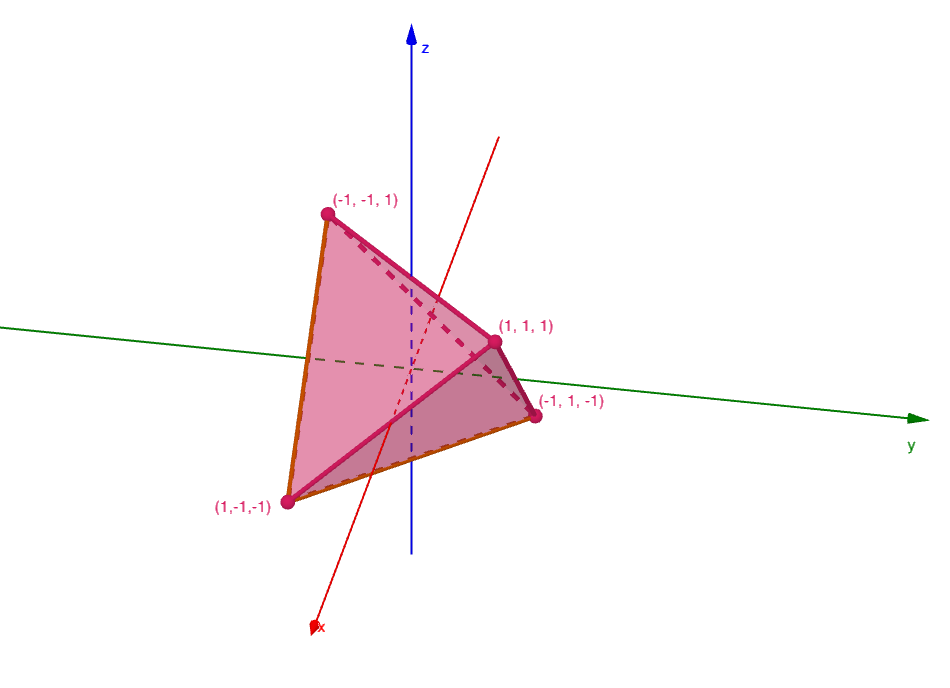
\includegraphics[width=0.6\textwidth]{images/polyeder/tetraederspeziellorientiert.png}
    \caption{Tetraeder mit Kanten $(1,1,1)$, $(1,-1,-1)$, $(-1,1,-1)$ und $(-1,-1,1)$.}
    \label{fig:tetraederspezielleorientierung}
\end{figure}
Wenn wir diese spezielle Ausrichtung des Tetraeders wählen, können wir die Rotationen um die Achsen von Typ $b$, siehe Abbildung \ref{fig:tetraederotationsachsen}, wie folgt darstellen:

\begin{align}
    A_0 = \begin{pmatrix} 1 & 0 & 0 \\ 0 & 1 & 0 \\ 0 & 0 & 1 \end{pmatrix}, \quad
    A_1 = \begin{pmatrix} 1 & 0 & 0 \\ 0 & -1 & 0 \\ 0 & 0 & -1 \end{pmatrix}, \nonumber \\
    A_2 = \begin{pmatrix} -1 & 0 & 0 \\ 0 & 1 & 0 \\ 0 & 0 & -1 \end{pmatrix}, \quad
    A_3 = \begin{pmatrix} -1 & 0 & 0 \\ 0 & -1 & 0 \\ 0 & 0 & 1 \end{pmatrix}. \nonumber
\end{align}
Die Rotation von Typ $a$ lässt sich mit der Matrix
\begin{align}
    R &= \begin{pmatrix} 0 & 0 & 1 \\ 1 & 0 & 0 \\ 0 & 1 & 0 \end{pmatrix} \nonumber
\end{align}
darstellen. Alle Abbildungen der Symmetriegruppe $T$ sind somit gegeben durch
$$ \left\{A_i R^k \mid k \in \{0,1,2\}, i \in \{0,1,2,3\} \right\}.$$
Somit können wir nun die Summe berechnen und wir erhalten
\begin{align}
    \sum_{w \in \Omega} \|\Pi_{E}w(s)\|^2  &= \sum_{k=0}^2 \sum_{i=0}^3 \|\Pi_{E}A_iR^k\|^2 \nonumber \\ 
    &=  \sum_{k=0}^2 \sum_{i=0}^3 \left\|\left(I - \begin{pmatrix}
        n_1^2 & n_1 n_2 & n_1 n_3 \\
        n_2 n_1 & n_2^2 & n_2 n_3 \\
        n_3 n_1 & n_3 n_2 & n_3^2
    \end{pmatrix}\right)A_iR^k\vec{s} \ \right\|^2  \nonumber \\
    &=8 \|\vec{s}\|^2, \nonumber
\end{align}
wobei wir die Tatsache benutzt haben, dass die Strecke $s$ unter Translation ihre Länge nicht verändert. Inbesondere, dass wir die Strecke $s$ auf den Ursprung verschieben können und dementsprechend $s$ als Vektor $\vec{s} \in \mathbb{R}^3$ betrachten können. 
\end{proof}
Wir möchten hier anmerken, dass das Ausmultiplizieren der Matrizen im Beweis keine schwierige, jedoch eine zeitintensive Aufgabe ist. Wir ermutigen die LeserInnen zumindest einmal die Rechnung selbst per Hand auszurechnen. Wie schon im Beweis erwähnt, folgen die Beweise für $\Omega \in \{H,I\}$ demselben Schema. Da die Kardinalität der Symmetriegruppen jedoch grösser ist, wird der Rechenaufwand dementsprechend auch grösser. Da kommt es gerade gelegen, dass wir anstatt die Summe der Kantenlängen unter der Orthogonalprojektion, siehe Gleichung \eqref{eq:sum_projection_independent_of_plane}, direkt auszurechnen, auch über die Irreduzibilität von den Symmetriegruppen den Beweis führen können.
\begin{proof}
    Sei $\vec{s} \in \mathbb{R}^3$ der Richtungsvektor der Strecke $s$. Wir nutzen die Zerlegung aus Gleichung \eqref{eq:vektor_parallel_senkrecht} und die Darstellung der Projektionslänge aus \eqref{eq:projectionwithvectorandnormal}. Für ein beliebiges $w \in \Omega$ gilt:
    \begin{align} 
        \|\Pi_{E}w(\vec{s})\|^2 &= \|w_{\parallel}(\vec{s})\|^2 \nonumber \\
        &= \|w(\vec{s})\|^2 - \|w(\vec{s})_{\perp}\|^2 \nonumber \\
        &= \|w(\vec{s})\|^2 - \|\left(\vec{n}_E \cdot w(\vec{s})\right)\vec{n}_E\|^2, \nonumber
    \end{align}
    wobei $\vec{n}_E$ der Normalenvektor der Ebene $E$ ist, d.h. $\|\vec{n}_E\| = 1$. Da alle Abbildungen $w \in \Omega$ Drehungen und somit Isometrien (längenerhaltend) sind, gilt $\|w(\vec{s})\|^2 = \|\vec{s}\|^2$. Summiert über die gesamte Gruppe ergibt sich:
    \begin{align} 
        \sum_{w \in \Omega} \|\Pi_{E}w(\vec{s})\|^2 &= \sum_{w \in \Omega} \left( \|w(\vec{s})\|^2 - \|\left(\vec{n}_E \cdot w(\vec{s})\right)\vec{n}_E\|^2 \right) \nonumber \\
        &= \sum_{w \in \Omega} \left( \|\vec{s}\|^2 - |\vec{n}_E \cdot w(\vec{s})|^2 \|\vec{n}_E \|^2\right) \nonumber \\
        &= |\Omega|  \|\vec{s}\|^2 - \sum_{w \in \Omega} |\vec{n}_E \cdot w(\vec{s})|^2. \nonumber
    \end{align}
    Der erste Term $|\Omega| \cdot \|\vec{s}\|^2$ ist konstant. Um die Unabhängigkeit bezüglich der Ebene $E$ zu zeigen, müssen wir nachweisen, dass auch der zweite Term konstant ist. Unter Verwendung der Identität $(\vec{a} \cdot \vec{b})^2 = \vec{a}^T(\vec{b} \ \vec{b}^T)\vec{a}$ erhalten wir:
    \begin{align} \label{eq:summevectormatrixnormal_revised}
        \sum_{w \in \Omega} |\vec{n}_E \cdot w(\vec{s})|^2 &= \sum_{w \in \Omega} \vec{n}_E^T \left( w(\vec{s}) w(\vec{s})^T \right) \vec{n}_E \nonumber \\
        &= \vec{n}_E^T \left( \sum_{w \in \Omega} w(\vec{s}) w(\vec{s})^T \right) \vec{n}_E.
    \end{align}
    Wir definieren die Matrix $$M := \sum_{w \in \Omega} w(\vec{s}) w(\vec{s})^T \in \mathbb{R}^{3 \times 3}.$$ 
        Das bedeutet, unsere Summe aus Gleichung \eqref{eq:sum_line_segment_projection_independent_of_plane} lässt sich wie folgt schreiben
       \begin{align} \label{eq:summemitmatrixM}
        \sum_{w \in \Omega} \|\Pi_{E}w(\vec{s})\|^2 = |\Omega|  \|\vec{s}\|^2 - \vec{n}_E^T M \vec{n}_E.
    \end{align}
    Nun stellt sich uns die Frage, wann der hintere Term konstant ist. Zuerst tragen wir jedoch zusammen, welche Eigenschaften die Matrix $M$ hat:
    \begin{itemize}
        \item[I.]  Die Matrix $M$ ist symmetrisch ($M=M^T$). Gemäss dem Spektralsatz, siehe Anhang \ref{sec:spektralsatzlinearealgebra}, besitzt die symmetrische Matrix $M$ einen reellen Eigenwert $\lambda$ mit zugehörigem Eigenraum $V_\lambda \neq \{0\}$.
        \item[II.] Die Matrix $M$ kommutiert mit jeder Drehung $R \in \Omega$:
    \begin{align}
        R M R^T &= \sum_{w \in \Omega} R w(\vec{s}) w(\vec{s})^T R^T = \sum_{w \in \Omega} (R w(\vec{s})) (R w(\vec{s}))^T= M, \nonumber
    \end{align}
 da die Multiplikation mit $R$ von links die Gruppenelemente lediglich permutiert. Wie wir bereits in Abschnitt \ref{sec:orthogonalrotation} gesehen haben, sind Drehungen orthogonal und es folgt 
 \begin{align} 
    RM = MR. \nonumber
 \end{align}
    \end{itemize}

 Für einen Vektor $\vec{v} \in V_\lambda$ gilt somit
    \begin{align}
        M(R\vec{v}) \overset{II.}{=} R(M\vec{v}) \overset{I.}{=} R(\lambda \vec{v}) = \lambda (R\vec{v}). \nonumber
    \end{align}
    Somit ist $R\vec{v} \in V_\lambda$, was bedeutet, dass $V_\lambda$ ein invarianter Unterraum unter der Wirkung von $\Omega$ ist. Da die Gruppen $T, H$ und $I$ nach Lemma \ref{lemma:irreduzibelsymmetriegruppen} irreduzibel auf dem $\mathbb{R}^3$ operieren, muss $V_\lambda = \mathbb{R}^3$ gelten. Daraus folgt, dass $M$ ein skalares Vielfaches der Einheitsmatrix ist: $$M = \lambda I_3.$$
    
    Eingesetzt in Gleichung \eqref{eq:summevectormatrixnormal_revised} ergibt sich:
    \begin{align}
        \sum_{w \in \Omega} |\vec{n}_E \cdot w(s)|^2 = \vec{n}_E^T (\lambda I_3) \vec{n}_E = \lambda (\vec{n}_E^T \vec{n}_E) = \lambda. \nonumber
    \end{align}
    Da $\lambda$ eine Konstante ist, ist die Summe der quadrierten Projektionslängen unabhängig von der Ebene $E$.
\end{proof}





Beachte, dass im Gegensatz zum direkten Beweis, der explizite Wert der Summe in Gleichung \eqref{eq:sum_line_segment_projection_independent_of_plane} nicht berechnet wird. Nun haben wir alles beisammen, um die Aussage in Satz \ref{satz:sum_projection_independent_of_plane} zu beweisen.

\begin{proof}
    Sei $P$ ein Polyeder mit Symmetriegruppe $\Omega = T, H$ oder $I$. TODO:...
\end{proof}

Beachte, dass der Tetraeder, Hexaeder und Ikosaeder alle nur eine Äquivalenzklasse haben. Um ein Objekt zu finden, welches eines der Symmetriegruppen $T$, $H$ oder $I$ hat und mehrere Äquivalenzklassen aufweist, braucht es etwas kreativität. Ein Beispiel ist das Chiral-Polyeder in Abbildung \ref{fig:chiralpolyeder}.
\begin{figure}[htp]
    \centering
    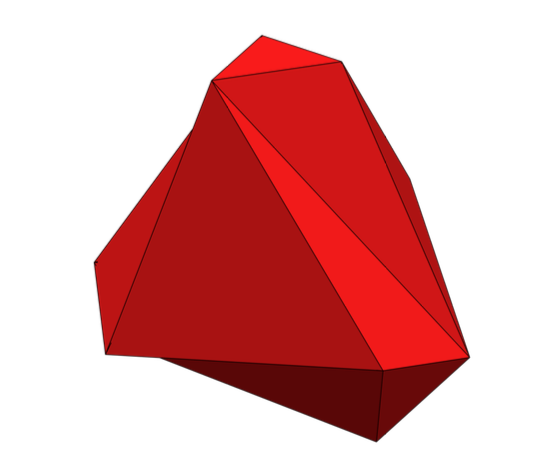
\includegraphics[width=10cm]{images/polyeder/chiral_polyeder.png}
    \caption{Ein Chiral-Polyeder mit Symmetriegruppe $T$, welches mehrere Äquivalenzklassen aufweist.\protect\footnotemark}
    \label{fig:chiralpolyeder}
\end{figure}
\footnotetext{Quelle: \cite{hungerbuehler_symmetric_polyhedra}}

\begin{example} \label{example:geradesprisma}
    Eine Frage, die man sich stellen könnte, ist, wieso der Beweis für Lemma \ref{lemma:quadriertesummeinvarianzstrecken} nicht für andere Symmetriegruppen funktioniert. Dafür betrachten wir zum Beispiel ein gerades Prisma mit einem $n$-Eck als Grunfläche, siehe Abbildung \ref{fig:geradesprisma}. 
    \begin{figure}[htp]
    \centering
    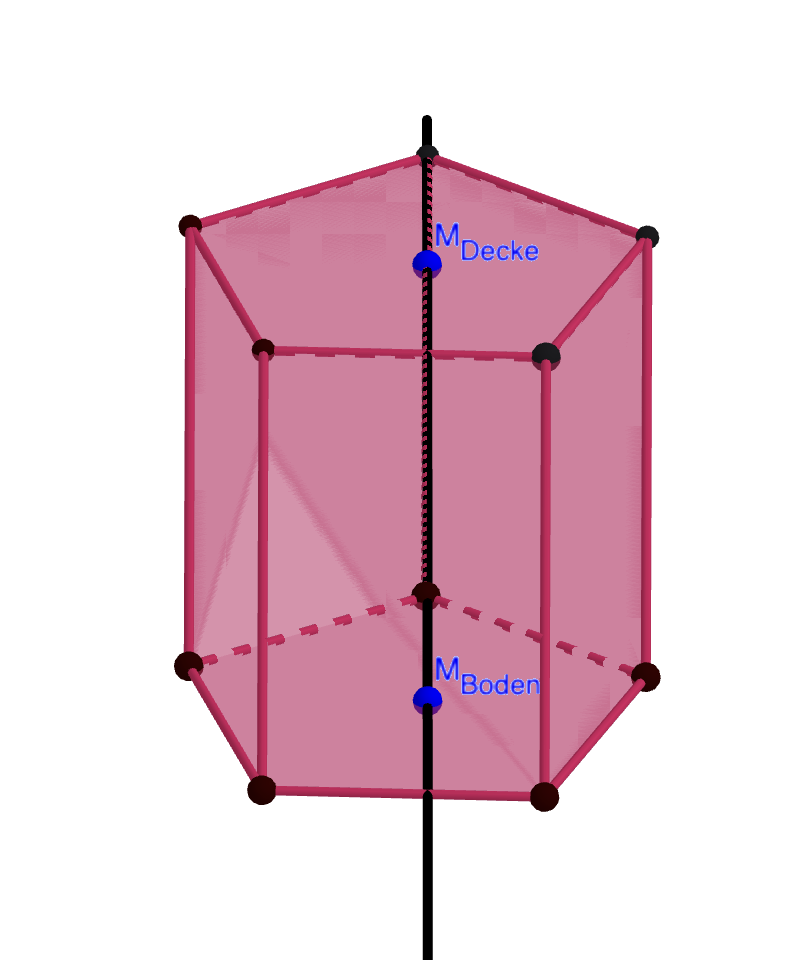
\includegraphics[width=0.4\textwidth]{images/prisma_z_achse.png}
    \caption{Gerades Prisma mit einem $5$-Eck als Grundfläche.}
    \label{fig:geradesprisma}
\end{figure}
    Die Symmetriegruppe vom geraden Prisma ist die \textit{Diedergruppe $D_n$}, welches die Symmetriegruppe des regulären $n$-Ecks ist. Die orientierungserhaltenden Kongruenztransformationen sind die Drehungen, um die Achse, welche durch die Mittelpunkte, $M_{\text{Boden}}$ und $M_{\text{Decke}}$ der $5$-Ecke verläuft (Sowie der achse durch eine Kante und mittelpunkt). Somit ist die z-Achse ein nicht-trivialer invarianter Unterraum $U \subset \mathbb{R}^3$ und folglich $D_n$ nicht irreduzibel. Somit würde der Beweis nicht mehr funktionieren. Stattdessen berechnen wir zuerst einmal die Matrix $M:= \sum_{w \in \Omega} w(\vec{s}) w(\vec{s})^T$. Beachte, dass wir in diesem Fall zwei Orbits haben: Die Höhenkanten sowie die Kanten vom $n-$Eck, am Boden sowie an der Decke. Das heisst für die Matrix $M$ gilt
    \begin{align}
        M = M_{\text{Höhenkanten}} + M_{\text{Kanten n-Eck}}. \nonumber
    \end{align}
    Für die Höhenkanten gilt 
    \begin{align}
        M_{\text{Höhenkanten}}=& \sum_{w \in D_n} \begin{pmatrix} 0 \\ 0 \\ h \end{pmatrix} \begin{pmatrix} 0 \\ 0 \\ h \end{pmatrix}^T \nonumber \\
        =& \begin{pmatrix} 0 & 0 & 0 \\ 0 & 0 & 0 \\ 0 & 0 & n  h^2 \end{pmatrix}. \nonumber 
    \end{align}
    Analog gilt
    \begin{align}
        M_{\text{Kanten n-Eck}} &= \sum_{w \in D_n}\begin{pmatrix} x_i \\ y_i \\ 0 \end{pmatrix} \begin{pmatrix} x_i & y_i & 0 \end{pmatrix} \nonumber \\
        &= n\begin{pmatrix} x_i^2 & x_i y_i & 0 \\ x_i y_i & y_i^2 & 0 \\ 0 & 0 & 0 \end{pmatrix} \nonumber \\
        &= \begin{pmatrix} n  a^2 & 0 & 0 \\ 0 & n  a^2 & 0 \\ 0 & 0 & 0 \end{pmatrix}. \nonumber
    \end{align}
    Es folgt
    \begin{align}
        M = \begin{pmatrix} n  a^2 & 0 & 0 \\ 0 & n  a^2 & 0 \\ 0 & 0 & nh^2 \end{pmatrix}. \nonumber
    \end{align}
    Daraus folgen zwei Fälle
    \begin{itemize}
        \item Fall $a \neq h$: $M \neq \lambda I_3 \implies $ Die Summe der quadrierten Kantenlängen unter eine Orthogonalprojektion sind nicht unabhängig von der Ebene.
        \item Fall $a = h$: $M = na^2 I_3 \implies $ Die Summe \eqref{eq:sum_line_segment_projection_independent_of_plane} bleibt, unabhängig von der Ebene, konstant.
    \end{itemize}
    Dies beendet unser Beispiel.
\end{example}


Eine interessante Beobachtung von Beispiel \ref{example:geradesprisma} ist, dass die Bedingungen in Satz (\ref{satz:sum_projection_independent_of_plane}) eine hinreichende, aber keine notwendige Bedingung ist für die Projektionseigenschaft (siehe Gleichung (\ref{eq:sum_projection_independent_of_plane})). Das heisst es existieren Polyeder, welche die Projektionseigenschaft erfüllen, aber nicht die Symmetrieeigenschaften besitzen. Ein Beispiel dafür ist das gerade Prisma mit $a=h$. Ein weiteres Beispiel ist der Pseudo-Rhombenkuboktaeder, siehe Abbildung \ref{fig:Pseudorhombicuboctahedron}. \footnote{Nicht zu verwechseln mit dem Rhombenkuboktaeder (siehe Abschnitt \ref{sec:rhombenkuboktaeder}).}

\begin{figure}[htp]
    \centering
    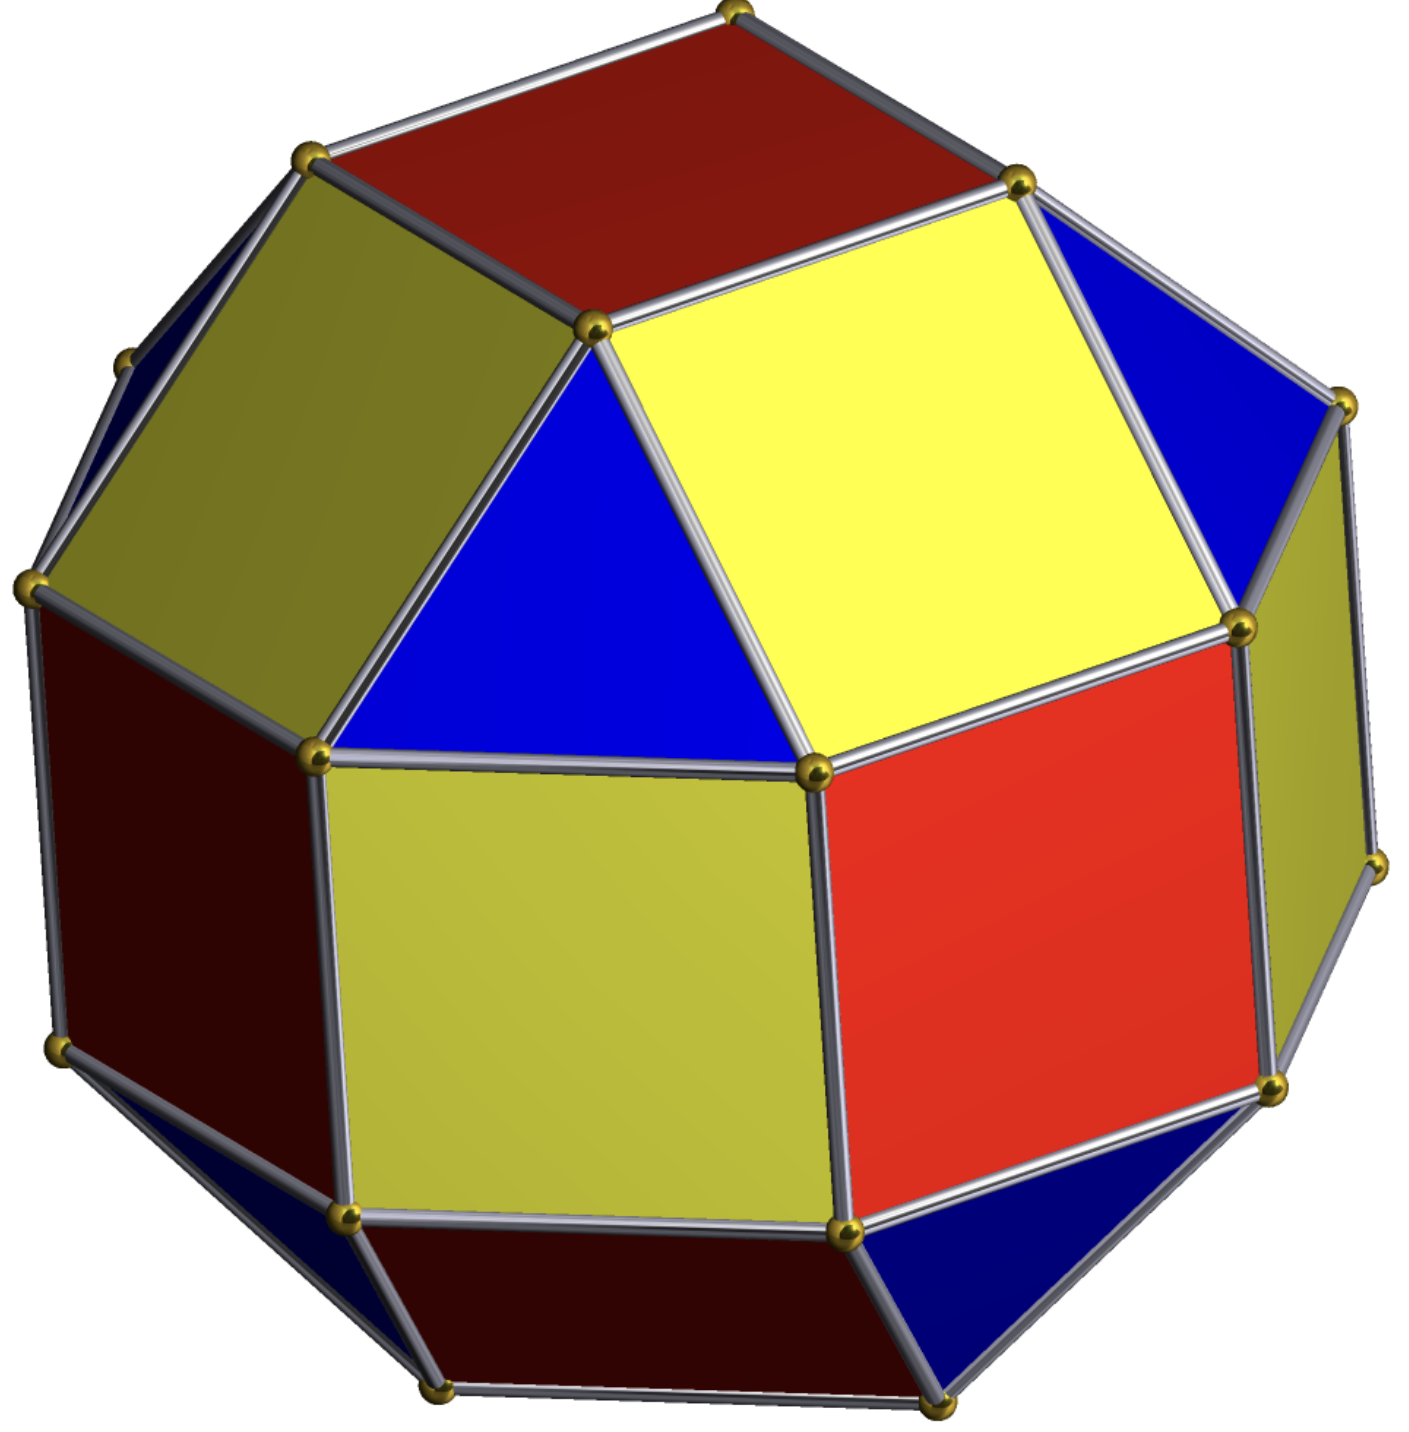
\includegraphics[width=10cm]{images/polyeder/Pseudorhombicuboctahedron.png}
    \caption{Pseudo-Rhombenkuboktaeder (elongated square gyrobicupola), Wikipedia \cite{elongated_square_gyrobicupola}.}
    \label{fig:Pseudorhombicuboctahedron}
\end{figure}
\begin{example} [Symmetriegruppe Pseudo-Rhombenkuboktaeder]
    Eine unserer Behauptungen ist, dass der Pseudo-Rhombenkuboktaeder keine der Symmetriegruppen T, H oder I hat. Wenn wir das Pseudo-Rhombenkuboktaeder (siehe Abbildung \ref{fig:Pseudorhombicuboctahedron}) betrachten, stellen wir fest, dass wir eine Symmetrieachse 4.\ Orndung haben. Diese geht vertikal durch das obere und untere rote Quadrat ("Deckel" und "Boden"). Da die Symmetriegruppe T gar keine Symmetrieachse 4.\ Ordnung hat, können wir ausschliessen, dass der Pseudo-Rhombenkuboktaeder die Symmetriegruppe T hat. Bemerke, dass das Pseudo-Rhombenkuboktaeder genau eine Symmetrieachse 4.\ Ordnung besitzt. Analog können wir auch die Symmetriegruppen H und I ausschliessen (siehe Aufgaben \ref{ex:PseudoRhombenkuboktaeder_Symmetriegruppe}).
\end{example}

Es bleibt also noch zu zeigen, dass das Pseudo-Rhombenkuboktaeder die Gleichung 
(\ref{eq:sum_projection_independent_of_plane}) erfüllt.

\begin{proposition}
    Sei $\Pi_{E}:\mathbb{R}^3 \rightarrow E$ die orthogonale Projektion auf eine Ebene $E \subset \mathbb{R}^3$. Dann ist die Summe der Quadrate der projizierten Kanten von einem Pseudo-Rhombenkuboktaeder $P$ unabhängig von der Ebene $E$, i.e. 
    \begin{align}
        \sum_{k \in K_{P}} ||\Pi_{E_1}(k)||^2 = \sum_{k \in K_P} ||\Pi_{E_2}(k)||^2 \quad .
    \end{align}
\end{proposition}
\begin{proof}
    TODO:...
\end{proof}

\newpage

\subsection{Polygone}

\begin{theorem} \label{satz:polygon_unabhängig_von_rotationswinkel}
    Sei $P$ ein Polygon in der Ebene $E_1 \subset \mathbb{R}^3$ mit Symmetriegruppe $C_n, n\geq 3$, und $\Tilde{P}$ die Abbildung einer Rotation mit Winkel $\mu$ von $P$ in der Ebene $E_1$. Zudem sei $\Sigma_{E_2}: \mathbb{R}^3 \rightarrow \Sigma_2$ die Orthogonalprojektion auf die Ebene $E_2 \subset \mathbb{R}^3$. Dann ist die Summe der Quadrate der Kantenlängen von der Projektion abhängig vom Winkel zwischen den beiden Ebenen $E_1$ und $E_2$ aber unabhängig vom Rotationswinkel $\mu$.
\end{theorem}

\begin{proof}
    TODO:...
\end{proof}

\subsection{Aufgaben}
\begin{exercise} [Äquivalenzklassen regulärer Hexaeder] \label{ex:äquivalenzklassen_regulärer_hexaeder}
Betrachten Sie einen regulären Hexaeder. Überlegen Sie sich wie viele Äquivalenzklassen der Tetraeder unter der Symmetriegruppe $H$ besitzt.
\end{exercise}

\begin{exercise} [Äquivalenzklassen] \label{ex:äquivalenzklassen}
Überlegen Sie sich ein Beispiel, welches mehrere Äquivalenzklassen besitzt.
\end{exercise}



\begin{exercise}[Symmetrie] \label{ex:notwendigkeitsymmetrie}
Gehen Sie nochmals durch den Beweis von Satz \ref{satz:sum_projection_independent_of_plane}. Können Sie erklären wo die Symmetriegruppeneigenschaft notwendig ist? Können Sie auch ein Beispiel nennen, wo diese Symmetrieeigenschaft nicht vorhanden ist und die Rechnung nicht aufgeht?
\end{exercise}

\begin{exercise} \label{ex:alternativbeweislemma}
Gehen Sie den Alternativbeweis zu Lemma (\ref{lemma:quadriertesummeinvarianzstrecken}) durch. \begin{itemize}
    \item[a)] Erklären Sie wieso aus 
\begin{align}
    M = \lambda I_3 \nonumber
\end{align}
folgt.
\item[b)] Berechnen Sie $\lambda$ für $\Omega=H$.
\end{itemize}
\end{exercise}

\begin{exercise}[Orthogonale Projektion] \label{ex:notwendigkeitorthogonaleprojektionen}
Gehen Sie nochmals durch den Beweis von Satz \ref{satz:sum_projection_independent_of_plane}. Erkläre in eigenen Worten, wo die orthogonal Projektionen verwendet werden im Beweis.
\end{exercise}
\begin{exercise}[Umkehrung] \label{ex:umkehrung_satz}
Gilt die Umkehrung von Satz \ref{satz:sum_projection_independent_of_plane}, d.h. falls Gleichung (\ref{eq:sum_projection_independent_of_plane}) gilt, folgt, dass $P \subset \mathbb{R}^3$ ein Polyeder mit Symmetriegruppe $T,H$ oder $I$ ist und wir eine orthogonale Abbildung haben.
\end{exercise}


\begin{exercise}  \label{ex:summe_einheitswurzel}
Zeige, dass für  $n \geq 3$ 

    \begin{align} \label{eq:summe_einheitswurzel}
        \sum_{k=0}^{n-1}e^{i4k\pi/n} = 0  
    \end{align}
gilt.
\end{exercise}


\begin{exercise} \label{ex:summ_einheitswurzel_smaller_than_3}
    Zeige, dass Gleichung (\ref{eq:summe_einheitswurzel}) für $n=1$ und $n=2$ nicht gilt.
\end{exercise}

\begin{exercise} \label{ex:PseudoRhombenkuboktaeder_Symmetriegruppe}
    Zeige, dass das Pseudo-Rhombenkuboktaeder weder Symmetriegruppe H noch I hat.
\end{exercise}